\documentclass[a4paper]{article}

\usepackage[swedish]{babel}
\usepackage[utf8x]{inputenc}
\usepackage{amsmath}
\usepackage{amssymb}
\usepackage[T1]{fontenc}
\usepackage{graphicx}
\usepackage{epstopdf}

\title{Komplettering}

\begin{document}

\maketitle

\section*{1.1}

Enligt uppgiften skall

\begin{equation*}
	v(x,y) = x^3 + axy^2 - 3x^2y + y^3
\end{equation*}

bestämmas som imaginärdelen av en holomorf funktion $f(z) = f(x + iy) = u + iv$. Eftersom $f$ skall vara holomorf så kommer $u$ och $v$ att vara harmoniska (enl. sats 3.22,) vilket medför att $\nabla^2v = v''_{xx} + v''_{yy} = 0$, där derivatorna ges av

\begin{align*}
	&\begin{cases}
		v'_x = 3x^2 + ay^2 - 6xy\\
		v'_y = 2axy - 3x^2 + 3y^2\\
	\end{cases}
	,\quad
	\begin{cases}
		v''_{xx} = 6x - 6y\\
		v''_{yy} = 2ax + 6y\\
	\end{cases}\\
	&\\
	&\nabla^2v = v''_{xx} + v''_{yy} = 0\\
	&\iff 6x - 6y + 2ax + 6y = 0\\
	&\iff x(6+2a) = 0\\
	&\implies a = -3.
\end{align*}

Till följd av Cauchy Riemanns ekvationer kan derivatan av $f$ skrivas som 

\begin{align*}
	f'(x + iy)	&= u'_x(x,y) + iv'_x(x,y) = v'_y(x,y) + iv'_x(x,y)\\
				&= (-6xy - 3x^2 + 3y^2) + i(3x^2 - 3y^2 - 6xy).\\
\end{align*}

Om sedan $x,y$ sätts till $x = z, y = 0$ respektive så kan derivatan skrivas som ett uttryck i enbart z

\begin{align*}
	f'(z) = -3z^2 + i3z^2
	\implies f(z) = \int f'(z)dz = -z^3 + iz^3 + C.
\end{align*}

Begynnelsevilkoret $f(0) = 1$ ger sedan att $C = 1$. $f$ blir då

\begin{equation*}
	f(z) = - z^3 + iz^3 + 1.
\end{equation*}

Uppgiften kan även lösas med Maple genom att först definiera $v(x,y)$ samt utnyttja att $v(x,y)$ är harmonisk för att lösa ut $a$.

\begin{figure}[h!]
	\centering
	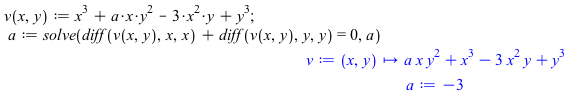
\includegraphics[width=0.9\textwidth]{maple_11_1.png}
\end{figure}

Sedan fås $u(x,y)$ genom att uttnyttja $u'_x = v'_y$ från Cauchy Riemanns ekvationer och integrera $v'_y$ med avseende på $x$ och sedan addera en funktion $h(y)$.

\begin{figure}[h!]
	\centering
	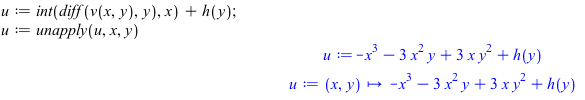
\includegraphics[width=0.9\textwidth]{maple_11_2.png}
\end{figure}

$h(y)$ fås sedan genom att lösa differentialekvationen $u'_y + v'_x = $, som återigen fås ur Cauchy Riemanns ekvationer.

\begin{figure}[h!]
	\centering
	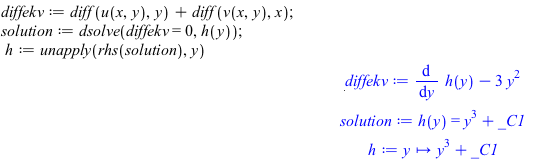
\includegraphics[width=0.9\textwidth]{maple_11_3.png}
\end{figure}

Funktionen $f(z) = f(x, y)$ kan sedan bildas genom att utnyttna det tidigare variabelbytet $x = z, y = 0$, och integrationskonstantens värde fås ur begynnelsevilkoret, precis som tidigare.

\begin{figure}[h!]
	\centering
	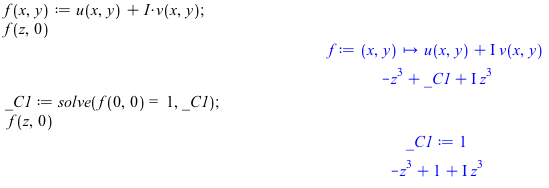
\includegraphics[width=0.9\textwidth]{maple_11_4.png}
\end{figure}

Vilket stämmer överens med det tidigare resultatet.

\section*{1.3}
\subsection*{c)}

På liknande vis som i förra deluppgiften används definitionen av den komplexa logaritmen för att utveckla uttrycket

\begin{align*}
	\text{Log}(e^z) = \ln|e^z| + i\text{Arg}(e^z)  = \ln(e^{|z|}) + i\text{Arg}(e^z) = |z| + i\text{Arg}(e^z) = 0.
\end{align*}

Den sista likheten gäller enligt uppgiften som gavs. Då måste $i\text{Arg}(z) = 0$ och $z$ måste ligga på den positiva reella axeln.

\section*{1.4}
\subsection*{b)}

Beräkna

\begin{equation*}
	\int_\gamma \frac{e^z}{z^2 + 4}, \gamma = x^2 + 4y^2 = 100.
\end{equation*}

Integranden är återigen uppbyggd av holomorfa funktioner och är då själv holomorf. Först undersöks nämnarens nollställen

\begin{align*}
	z^2 = -4 \implies z = \pm 2i,
\end{align*}

Nollställena ligger båda innanför området som omsluts av $\gamma$, integranden kan då delas upp med partialbråksuppdelning efter vilket Cauchys Integralformel kan användas för att beräkna kurvintegralen på varje delområde (som nu endast innehåller en singularitet).

\begin{align*}
	&\frac{e^z}{z^2 + 4} = \frac{e^z}{(z-2i)(z+2i)} = \frac{A}{z-2i} + \frac{B}{z+2i} = \frac{Az + i2A + Bz - i2B}{z^2 + 4}\\
	&\implies	\begin{cases}
					A = B\\
					2Az = e^z \implies A = e^z/2z = B
				\end{cases}.
\end{align*}

Integralen kan då skrivas som

\begin{align}
	\int_\gamma \frac{e^z}{z^2 + 4} = \int_\gamma \frac{\frac{e^z}{2z}}{z-2i}dz + \int_\gamma \frac{\frac{e^z}{2z}}{z+2i}dz.\label{eq:uppdelad}
\end{align}

Sätt $f(z) = \frac{e^z}{2z}$, då kan den uppdelade integralen i (\ref{eq:uppdelad}) skrivas som

\begin{align*}
	(\ref{eq:uppdelad}) &\iff \int_\gamma \frac{f(z)}{z-2i}dz + \int_\gamma \frac{f(z)}{z+2i}dz\\
		&= 2\pi i f(2i) + 2\pi i f(-2i) = 2\pi i \frac{e^{2i}}{4i} - 2\pi i \frac{e^{-2i}}{4i}\\
		&= i\pi\frac{(e^{2i} - e^{-2i})}{2i} = i\pi\sin 2.
\end{align*}

\subsection*{1.6}

Lös rekursionsekvationen

\begin{equation}
	\begin{cases}
		x_{n} - 10x_{n-1} + 50x_{n-2} = 0, n = 2,3,...\\
		x_0 = x_1 = 10
	\end{cases}\label{eq:rek_ekv_2}.
\end{equation}

Den homogena ekvationen (\ref{eq:rek_ekv_2}) har följande utseende

\begin{align*}
	1 - 10r^{-1} + 50r^{-2} = 0 &\iff 1 - \frac{10}{r} + \frac{50}{r^2} = 0\\
								&\iff r^2 - 10r + 50 = 0\\
								&\implies	\begin{cases}
												r_1 = 5 + 5i\\
												r_2 = 5 - 5i
											\end{cases}.
\end{align*}

Eftersom den karakteristiska ekvationen har två separata nollställen så ges lösningen till den homogena ekvationen av (enl. sats 4.14)

\begin{equation*}
	x_n = C_1r_1^n + C_2r_2^n
\end{equation*}
	
Begynnelsevilkoren ger sedan värdet på konstanterna $C_1$ och $C_2$

\begin{align*}
	\begin{cases}
		x_0 = 0\\
		x_1 = 10
	\end{cases}
	&\iff
	\begin{cases}
		C_1 + C_2 = 0\\
		C_1r_1 + C_2r_2 = 10
	\end{cases}\\
	&\iff
	\begin{cases}
		C_2 = -C_1\\
		C_1r_1 - C_1r_2 = 10
	\end{cases}\\
	&\implies C_1 = \frac{10}{r_1 - r_2} = \frac{10}{10i} = \frac{1}{i} = -i\\
	&\implies C_2 = i
\end{align*}

Lösningen kan då skrivas som

\begin{align*}
	x_n		&= -i(5+5i)^n + i(5-5i)^n\\
			&= -i(5(1+i))^n + i(5(1-i))^n\\
			&= -i(5\sqrt{2}e^{i\frac{\pi}{4}})^n + i(5\sqrt{2}e^{i-\frac{\pi}{4}})^n\\
			&= -i5^n\sqrt{2}^n(e^{i\frac{\pi}{4}n} - e^{-i\frac{\pi}{4}n})\\
			&= -i\sqrt{50}^n\sin\left(\frac{\pi}{4}n\right)2i\\
			&= 2\cdot\sqrt{50}^n\sin\left(\frac{\pi}{4}n\right)
\end{align*}

Värdet på $x_{32}$ beräknas i Maple samt Matlab.

\begin{figure}[h!]
	\centering
	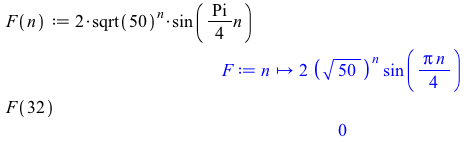
\includegraphics[width=0.75\textwidth]{maple.png}
	\caption{Utskrifter från Maple vid beräknings av $x_{32}$}
	\label{fig:maple}
\end{figure}

\begin{figure}[h!]
	\centering
	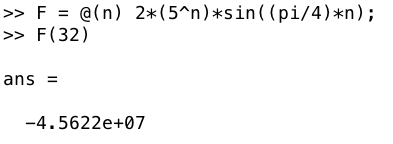
\includegraphics[width=0.75\textwidth]{matlab.png}
	\caption{Utskifter från Matlab vid beräknings av $x_{32}$}
	\label{fig:matlab}
\end{figure}

Beräknas $x_{32}$ istället för hand fås

\begin{equation*}
	x_{32} = 2\cdot5^{32}\sin\left(\frac{\pi}{4}n\right) = 2\cdot5^{32}\cdot 0 = 0.
\end{equation*}

Anledningen till varför resultatet skiljer så mycket för Matlab beror troligtvis på att programmet använder numeriska metoder för att approximera $\sin(x)$. I Figur \ref{fig:matlab} blir $\sin(8\pi)$ troligtvis mycket nära $0$, nog nära för att det inte skall spela roll i de flesta sammanhang, men i beräkningen av $x_{32}$ multiplicerar vi ett mycket stort tal $5^{32}$ med något som är nära noll och resultatet blir då $-4.6\cdot10^7$. Det här problemet grundar sig i att datorer idag och Matlab i synnerhet använder sig av 64 bitar för att representera ett decimaltal. Det betyder att det finns en fix precision för heltalsdelen och decimaldelen av ett tal och detta leder till fel vid multiplikation av tal som skiljer sig många storleksordningar. Dock verkar Maple använda sig av mer analytiska metoder för att beräkna $\sin(x)$ och leder därför inte av samma problem.

\end{document}
